\documentclass{article}
\usepackage{natbib}
\usepackage{graphicx}
\usepackage[colorlinks = true,
            linkcolor = blue,
            urlcolor  = blue,
            citecolor = blue,
            anchorcolor = blue]{hyperref}
\usepackage[utf8]{inputenc}
% Anonymize PDF
\pdfinfo{
  /Title ()
  /Creator ()
  /Producer ()
  /Author ()
  /Subject ()
  /Keywords ()
}

\title{Muskoin Protocol}
\author{\href{http://www.twitter.com/MuskoinApp}{@MuskoinApp} and \href{http://www.twitter.com/Muskrat42069}{@Muskrat42069}}
\date{April 2021}

\begin{document}

\maketitle

\begin{abstract}

Muskoin is an ultra-minimal, open source interface and protocol for bestowing eternal glory to authors of dank memes.

\end{abstract}

\section{Motivation}
The advent of modern social media platforms has made it possible for a single individual to connect with a global audience in a matter of seconds. Online ecosystems 
such as Twitter, Facebook, Reddit, etc. have changed the way we view the world and our place in it. An entertaining, yet unintended, side effect that has arisen from 
the widespread use of such platforms has been the phenomenon of viral \href{https://en.wikipedia.org/wiki/Meme}{memes}. Memes are a new, yet well-established, form of expression. This medium combines visual and written elements into a work that, along with temporal and societal context, can quickly communicate a complex set of ideas or shared experiences that 
are typically humorous in nature (though not necessarily). 

Thousands - or likely millions - of memes have been created and shared over the Internet in the last 15 years. Often, memes are shared so many times and experience so many mutations
that the original instance in which the meme was created is lost. \href{https://knowyourmeme.com/ }{Attempts} have been made to catalogue the provenance and evolution of the most popular or wide-spread specimens. However, due to the very nature of memes (their fast replication and evolution), the task of indexing their creation and attributing authorship is quite daunting. The intellectual creator of a viral meme has little recourse in claiming any kind of economic benefit from its genesis, even if their \href{https://en.wikipedia.org/wiki/Bad_Luck_Brian}{physical likeness} is used as
part of the meme's visual component. 

Blockchain technology has ushered in a new paradigm of digital ownership. Platforms like \href{https://ethereum.org/en/}{Ethereum} have even made it possible 
to execute arbitrary computational logic over a decentralized network of computers in a 
\href{https://www.nananke.com/single-post/2018/08/07/zero-trust-vs-trustless-systems}{trustless} fashion through the use of 
\href{https://en.wikipedia.org/wiki/Smart_contract}{smart contracts}. By leveraging smart contracts, it is now possible to create 
\href{https://www.investopedia.com/terms/f/fungibility.asp}{non-fungible} digital assets and assign irrefutable ownership of such assets. To this end, the 
\href{https://muskoin.app}{Muskoin protocol} is designed to facilitate a non-fungible digital representation of the authorship of a meme and at the same 
time, index its first appearance on the web.

\section{Technical Implementation}
The Muskoin Protocol is based on the ERC-721 non-fungible token (NFT) standard. Each NFT minted consists of an owner address and a token URI which permanently and immutably stores the hosting location of a meme on the Internet. 

The smart contract (Muskoin.sol) which contains the data-structures representing the NFTs is deployed to the Ethereum Mainnet. The smart contract itself contains two roles: MINTER\_ROLE and MINTER\_ADMIN\_ROLE. Upon initial deployment of the Muskoin.sol contract, the deployment wallet address is a member of both of these roles. The MINTER\_ADMIN\_ROLE has the authority to add new wallet addresses to the MINTER\_ROLE list. Only wallet addresses included in the MINTER\_ROLE list are allowed to issue new Muskoin NFTs. Members of either role can renounce their position by making a transaction call to the 'renounceRole' member function of Muskoin.sol. 

The user interface that allows interaction with the deployed Muskoin.sol contract is a React-based web application hosted on IPFS via the fleek.co service. We borrowed heavily from the Uniswap project for our first implementation of the Muskoin dApp and welcome proposed improvements from the community to our Github repository. 

\section{Governance}

Our intention for Muskoin Protocol is for it to be self-sustaining and for only a single individual, Elon Musk, to have the sole right to mint new Muskoin NFTs. Upon the event of Elon Musk sending his public wallet address to us, we will add his wallet address to the MINTER\_ROLE list, and renounce our position as MINTER\_ROLE. However, we intend to retain the MINTER\_ADMIN\_ROLE in case Elon loses access to the private key associated with the MINTER\_ROLE previously granted to him. 

All roles are easily audited by the community via a simple query to a blockchain scanning service such as Etherscan.

In order to serve as an irrefutable identification of our Twitter accounts associated with the Muskoin Protocol, the first two Muskoin NFTs will be minted such that their URIs will point to our respective Twitter pages. The subsequent two Muskoin NFTs will be minted to point to the official URLs of the Muskoin project, i.e. \href{http://muskoin.ceo}{http://muskoin.ceo} and \href{http://muskoin.app}{http://muskoin.app}. No further Muskoin NFTs will be minted from our actions after these initial four NFTs are created. 

\section{Conclusion}

This work is dedicated to the memory of our friend, Harambe. 

\begin{figure}[h!]
\centering
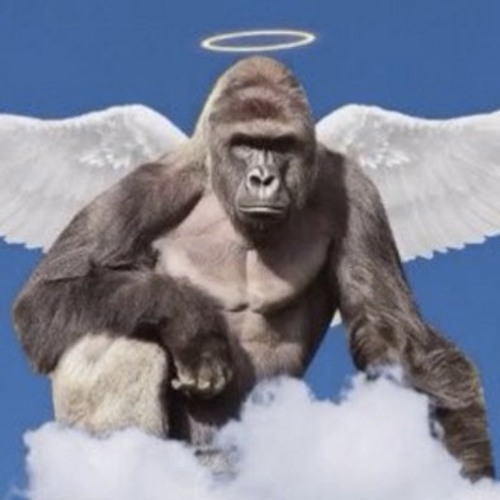
\includegraphics[scale=0.5]{harambe.jpg}
\caption{Harambe}
\label{fig:Harambe}
\end{figure}

\end{document}
